%!TEX root = ../main.tex
\chapter{Background Study}
\label{background}
\section {Overview}
This section will show other areas which required further research to aid in making a concrete decision as to which technology will be used for the development of the project.
\subsection{OS}
The majority of the apps on our mobile phones are native apps, meaning they are written in languages that the platform accepts, for example swift is used to write iOS apps and java is used to write Android apps while c\# is used for most Microsoft phone apps.
Native apps are very responsive and also offer the most reliable experience to user. On the other hand an hybrid app is more similar to a web app but is installed like a native app. They are normally built with javascript, HTML, and CSS and runs in something called webview, a browser within the app. Performance wise, however, it's inferior compared to native apps. 

The project was developed as a native app, using the Android OS, this was chosen based on the fact the author has knowledge of the platform and it is the OS with the largest share on the market, \cite{WebHybri87:online}.

\subsection{Database}
MYSQL was chosen as the database for this project, mainly for its scalability and its compatibility with Java and PHP language. For this reason phpMyAdmin was used aswell as a development tool to handle database management.

\section{Development Environment}
Relying on tools to develop an app is very useful as it helps accelerate the development. For Android there are various tools which this chapter will focus on describing.
To be able to build the application a development environment, Java Development Kit(JDK) and Android SDK are required.
To develop with the SDK, Google offers a bundle, the bundle comes with an IDE and the  Android SDK.

\subsection{JDK}
Java Development Kit is the essence of any java application. As defined by the Technopedia Dictionary, \say{the JDK is a software development environment used for developing Java applications and applets. It includes the Java Runtime Environment (JRE), an interpreter/loader (java), a compiler (javac), an archiver (jar), a documentation generator (javadoc) and other tools needed in Java development}.

\subsection{SDK}
Android Software Development Kit provides a selection of tools and libraries required to build Android apps to ensure the process goes as smoothly as possible and the SDK is used to get it to run on an Android device and access unique features of the OS.

\subsection{Android Emulator}
The emulator allows to run the app without having to install the app on an actual Android device. It emulates most of the functionality of a real Android device, apart from for the
GPS module. 
\begin{figure}[h]
	\centering	
	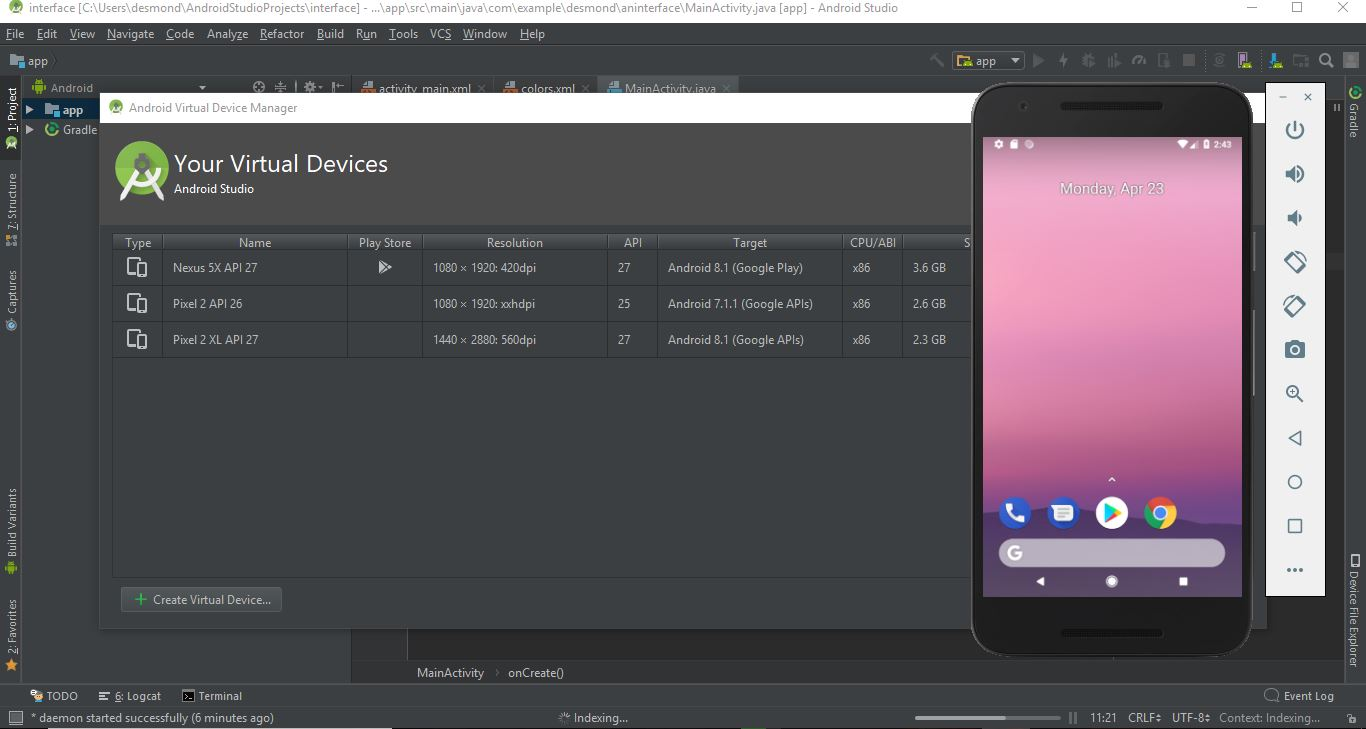
\includegraphics[width=0.5\textwidth]
	{emulator_view}
	\caption{Android Emulator}
	\label{fig:android_emulator}	
\end{figure}

\subsection{Graphic Layout}
The Layout Editor from the SDK allows developers to create user interfaces(UI) with an editor(Drag and Drop) or by writing XML Code. These editors support many features for rapid UI development and both are easy to use and it is directly included into Android Studio. The screen of the editor is shown in figure \ref{fig:android_ui_editor}.
\begin{figure}
	\centering
	\begin{subfigure}[h]{0.5\textwidth}  	      
		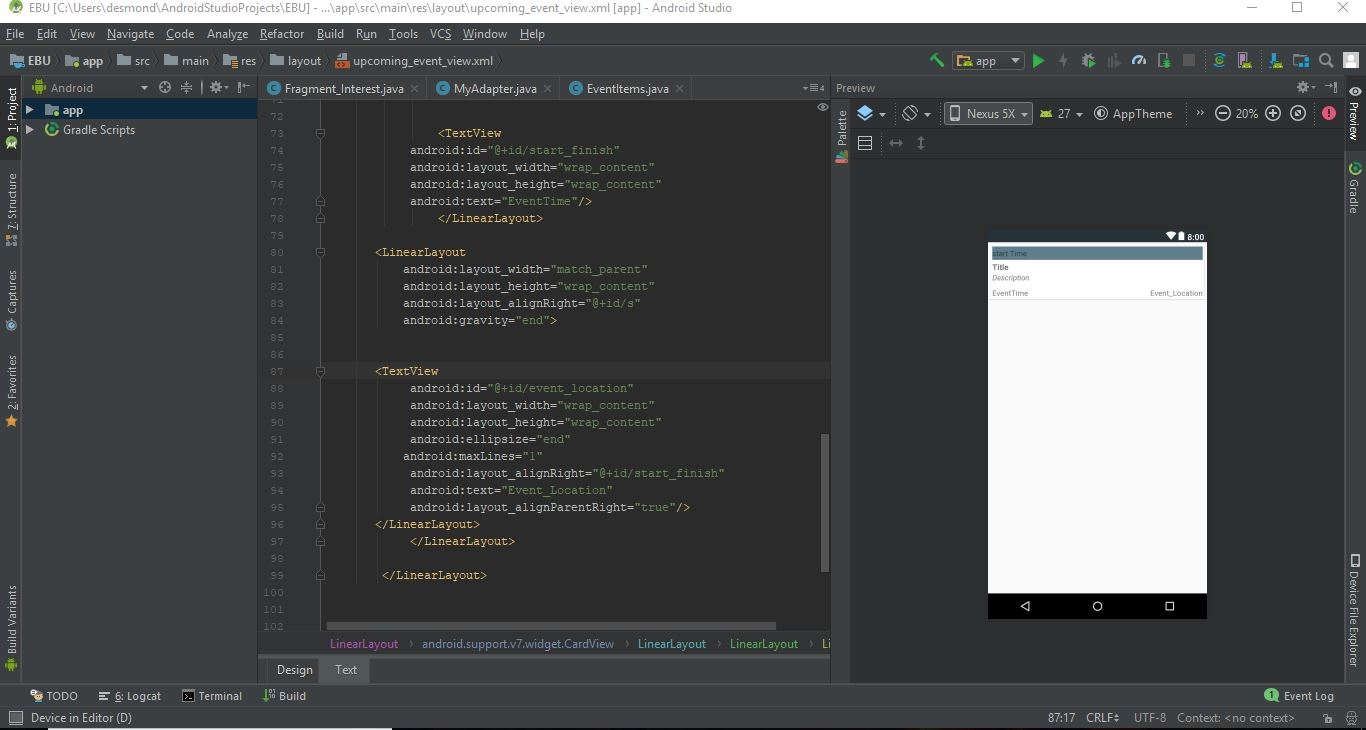
\includegraphics[width=.96\linewidth]{xml_text_view}
		\caption{XML Text View Editor}
		\label{fig:design_editor}
	\end{subfigure}%
	%add desired spacing between images, e. g. ~, \quad, \qquad etc.
	%(or a blank line to force the subfigure onto a new line)
	\begin{subfigure}[h]{0.5\textwidth}	
		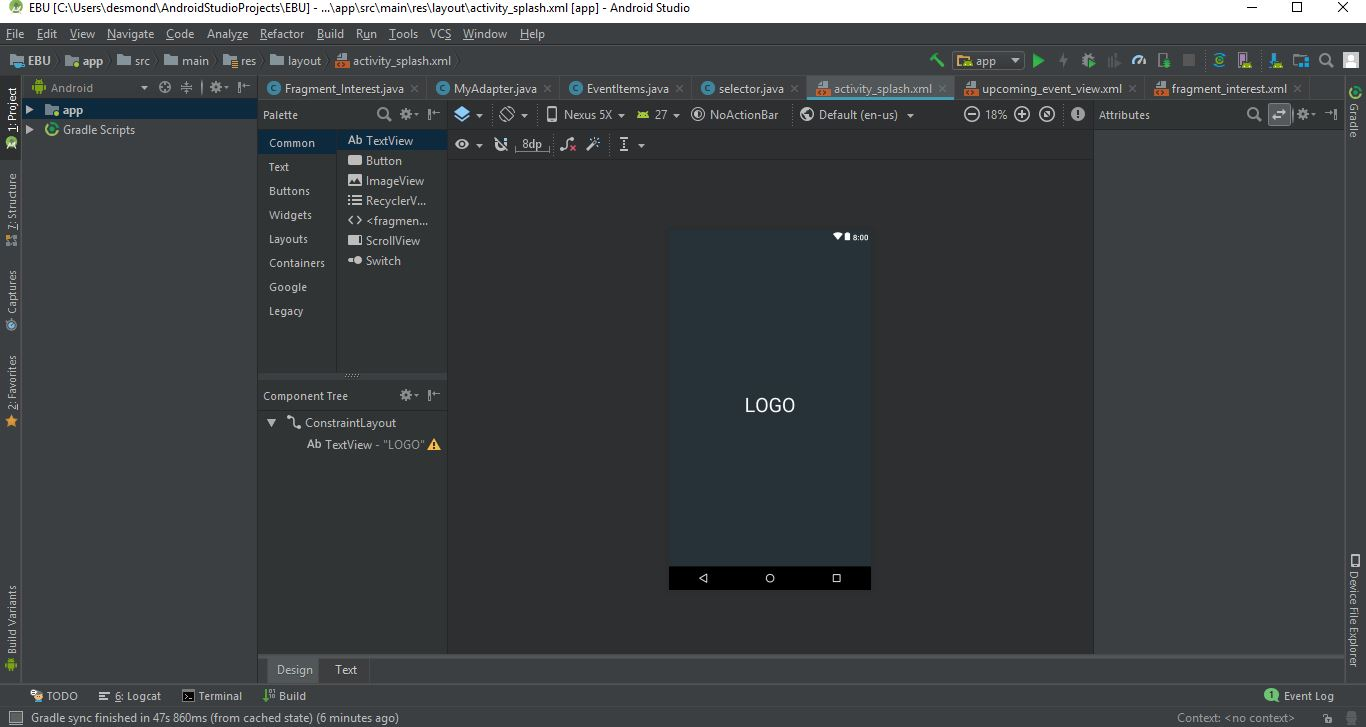
\includegraphics[width=.96\linewidth]{xml_design_view}
		\caption{XML Design View Editor}
		\label{fig:xmlEditor}
	\end{subfigure}
	\caption{Andriod UI Design Editor}\label{fig:android_ui_editor}
\end{figure}

\subsection{IDE}
According to TechTarget Integrated Development Enviroment(IDE) is \say{a software suit that consolidates the basic tool developers needs to write and test software. An IDE consists of a code editor, a compiler or interpreter and a debugger that the developer can access through a single graphical user interface}.
For the purpose of this project Android studio was used as its the official IDE for Android development.

\section {Android Framework and API}
In order to build the artefact, it is essential for the author to understand the Android framework and API, this information is found in Appendix \ref{framework}.


\section{Developing Problem}
Dealing with diverse platform is on of the most challenging aspect in app development. Mobile development is moving towards fragmentation rather than unification.

\textbf{Fragmentation:} Considering Android devices, most of them comes with different screen resolution. Different devices exist with different properties such as  CPU speed and memory. According to a study made by Mona, Ali and Phillipe in their article “Real Challenges in Mobile app Development”; 76\% of their survey participants see the existence of multiple platform as a challenge for developing mobile apps, while 23\% believe it is an opportunity for technology advances that drive innovation. The development process cannot leverage knowledge from a platform to another. Also, when an application is created for various platforms, the developers must treat the development independently  and check that consistency is kept across each one.
